\documentclass[compress]{beamer}
\useoutertheme[footline=authorinstitutetitle]{miniframes}
\usecolortheme{whale}
\usecolortheme{orchid}
\useinnertheme{rounded}

\setbeamerfont{block title}{size={}}

%\usepackage{beamerthemeproyxetex}
%\usepackage{synttree}

\title{COLIBRI: Constructions as Linguistic Bridges}
\author{Maarten van Gompel, Radboud University Nijmegen}
\date{FLARN - Tilburg University - March 2012}
\usepackage{graphicx}
\usepackage{placeins}



\def\raccoon{
\makebox[\linewidth][c]{\includegraphics[width=70pt]{/home/proycon/Pictures/All/raccoon.pdf}\FloatBarrier}
}
\def\smallraccoon{
\makebox[\linewidth][c]{\includegraphics[width=30pt]{/home/proycon/Pictures/All/raccoon.pdf}\FloatBarrier}
}

\begin{document}

\begin{frame}
	\titlepage\smallraccoon
\end{frame}

\section{Introduction}

\begin{frame}{Introduction}

	\begin{block}{Research objective}
		\textbf{Research objective:} Identification and extraction of ``good'' constructions in parallel corpus data.
	\end{block}

	\begin{block}{About the research}
		\begin{itemize}
			\item \textbf{Implicit Linguistics}: Deducing linguistic knowledge from corpus data
			\item Beyond n-gram models
			\item What is ``good''?
		\end{itemize}
	\end{block}
\end{frame}

\section{Constructions}

\begin{frame}{Constructions}

	\begin{block}{What is a construction?}
		\textbf{What is a construction?}  \\
		\begin{itemize}
			\item A \emph{pattern} of words, not necessarily consecutive,  which \emph{in some way} forms an entity
			\item Constructions emerge from the data rather than linguistic theory
			\item Intuitive ``building blocks'' for various NLP tasks
			\item A level above n-gram models and below syntactic level.
		\end{itemize}
	\end{block}

	 
\includegraphics[width=30.0mm]{lego.jpg}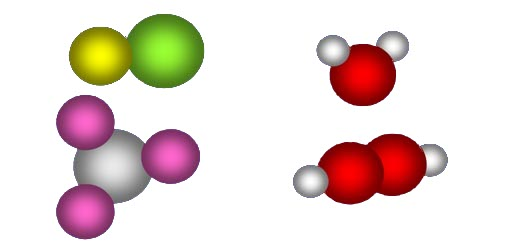
\includegraphics[width=40.0mm]{molecules.jpg} 
\end{frame}


\begin{frame}{Emerging constructions}
	Constructions emerge from the corpus data rather than from linguistic theory:
	\begin{enumerate}
		\item by frequency
		\item by context
		\item \textbf{by multilingual alignment}
	\end{enumerate}
\end{frame}


\begin{frame}{Counting patterns}
	\begin{itemize}
		\item Iterative counting, first unigrams, then bigrams
		\item  ... discarding pattern candidates if a sub-part was not found
		\item Counting constructions with gaps: \emph{``to be * to be''}
		\item ...by punching all combinations ``holes'' in found consecutive constructions
	\end{itemize}
\end{frame}

\section{Machine Translation}

\begin{frame}{Phrases as constructions in Machine Translation}
	%Constructions used as building blocks in MT
	%Multilingual alignment
	\begin{center}
		 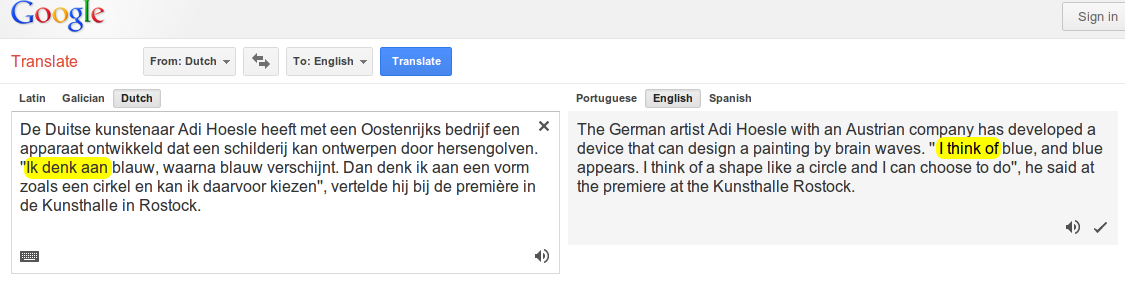
\includegraphics[width=110.0mm]{google1.png} 
	\end{center}
\end{frame}

\begin{frame}{Phrases as constructions in Machine Translation}
	%Constructions used as building blocks in MT
	%Multilingual alignment
	\begin{center}
		 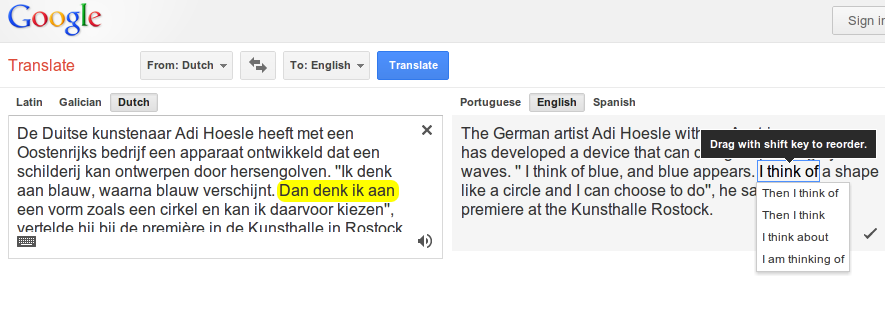
\includegraphics[width=110.0mm]{google2.png} 
	\end{center}
\end{frame}

\begin{frame}[fragile]
	\begin{block}{How are these relations accross languages found?}
		\textbf{How?} \emph{Measures of co-occurrence} \\
	\end{block}

	\begin{center}
	 
\includegraphics[width=45.0mm]{align1.png} 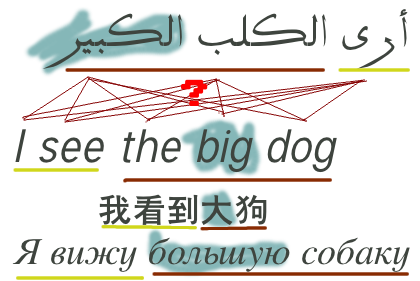
\includegraphics[width=45.0mm]{align2.png} 
	\end{center}
\end{frame}


\begin{frame}[fragile]
	\begin{example}	
		\begin{tabular}{l|l}
			'Uraa al-kalba al-kabira & I see the big dog \\
			'Uraa al-qitta al-saghira & I see the small cat	\\
			'Uraa al-qitta al-kabira & I see the big cat	\\
			akala al-rajul & The man ate \\
			Yuhabbu al-rajul al-qitta &  The man loves the cat \\
		\end{tabular} \\	

	\end{example}
	
	\smallskip
	\begin{center}
	\textbf{Try!} \\ \emph{'uraa?} \\
	\emph{al-kalba?} \\
	\emph{al-qitta al-saghira?} \\
	\emph{al-rajul?} \\
	\emph{yuhabbu?} \\
	\end{center}

\end{frame}

\begin{frame}[fragile]
	Excerpts of automatic alignment:

	\footnotesize{
	\begin{tabular}{l|l|l}
	\hline
	als lid	& as a member &	0.09 \\
	wil benadrukken dat	& want to emphasise that &	0.0493827 \\
	vrije verkeer van personen	& the free movement of persons &	0.140625	 \\
	tijdschema &	timetable &	0.237954 \\
  	Dat wil zeggen dat & This means that the & 0.0277778 \\
	\hline
	vertrouwen van de &	consumer confidence & 0.16	 \\
	\'e\'en enkele & single Member State & 0.0277778 \\
	oplossing van het &	the conflict &0.0219479 \\
	\hline
	goed voorstel &	to get this	& 0.01 \\
	Er bestaan &	of mobile &	0.0123457 \\
	\end{tabular}
	}
\end{frame}





\begin{frame}
	\begin{block}{MT Approaches}
		\begin{enumerate}
			\item \textbf{Rule-based:} explicit linguistic knowledge
			\item \textbf{Data-driven:} implicit linguistics	
			\begin{itemize}
				\item Statistical/machine learning models
			\end{itemize}						
		\end{enumerate}
	\end{block}

	\begin{block}{Two important aspects of translation}
		\begin{enumerate}
			\item Faithful conservation of meaning: good mapping between constructions
			\item Fluent natural style: natural word-order
		\end{enumerate}
	\end{block}
\end{frame}


\begin{frame}
	\begin{block}{What are the units of translation? $\rightarrow$ constructions }
		\begin{itemize}
			\item Whole sentences at once? No \\
			\item Single words, word by word? No \\
			\item Words in context? Better \\
			\item Variable-length phrases in context? Even better \\
			\item Loosening constraints: ``constructions'' in context? Best? \\
		\end{itemize}
	\end{block}

	\begin{center}
		 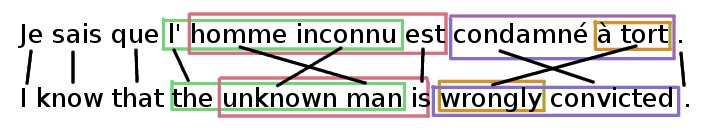
\includegraphics[width=90.0mm]{pbmbmt_alignment1c.jpg} \\
		 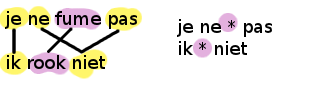
\includegraphics[width=50.0mm]{skipgram.png}
	\end{center}
\end{frame}


\section{Relations between Constructions}

\begin{frame}
	\begin{block}{Relations}		
		\begin{itemize}
			\item Relations between constructions from different languages
			\item Relations within constructions of the same language
		\end{itemize}
	\end{block}

	\begin{example}
		``I see the dog move''
		\begin{itemize}
			\item \textbf{Subsumption:}   ``I'' is a sub-part of `'I see''
			\item \textbf{Succession:}	  ``see`` is a successor of ``I''
			\item \textbf{Instantiation:}   ``I see the dog move'' instance of ``I see * move''
		\end{itemize}
	\end{example}
\end{frame}

\begin{frame}{Subsumption relations}
  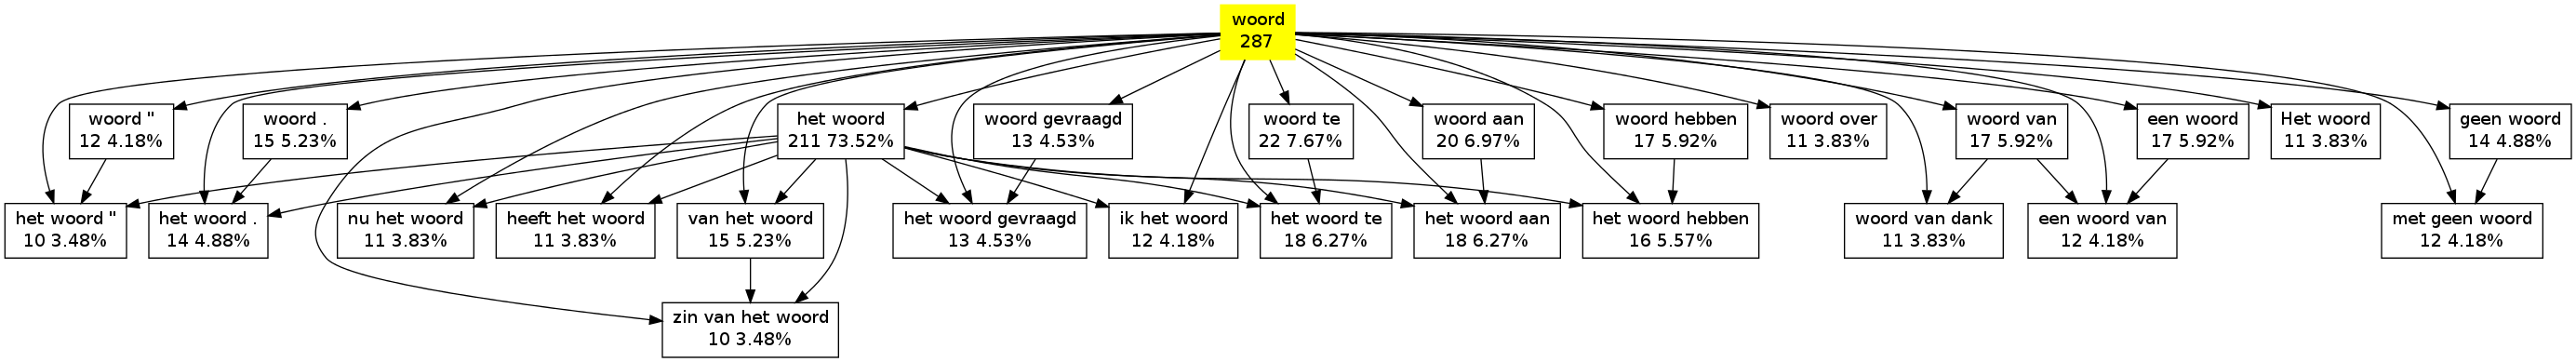
\includegraphics[width=160.0mm]{graph_woord_P.png}
\end{frame}

%\begin{frame}{Using subsumption relations to constrain constructions}
% \includegraphics[width=140.0mm]{graph_woord_X.png}
%\end{frame}

\begin{frame}{All relations: ``woord''}
 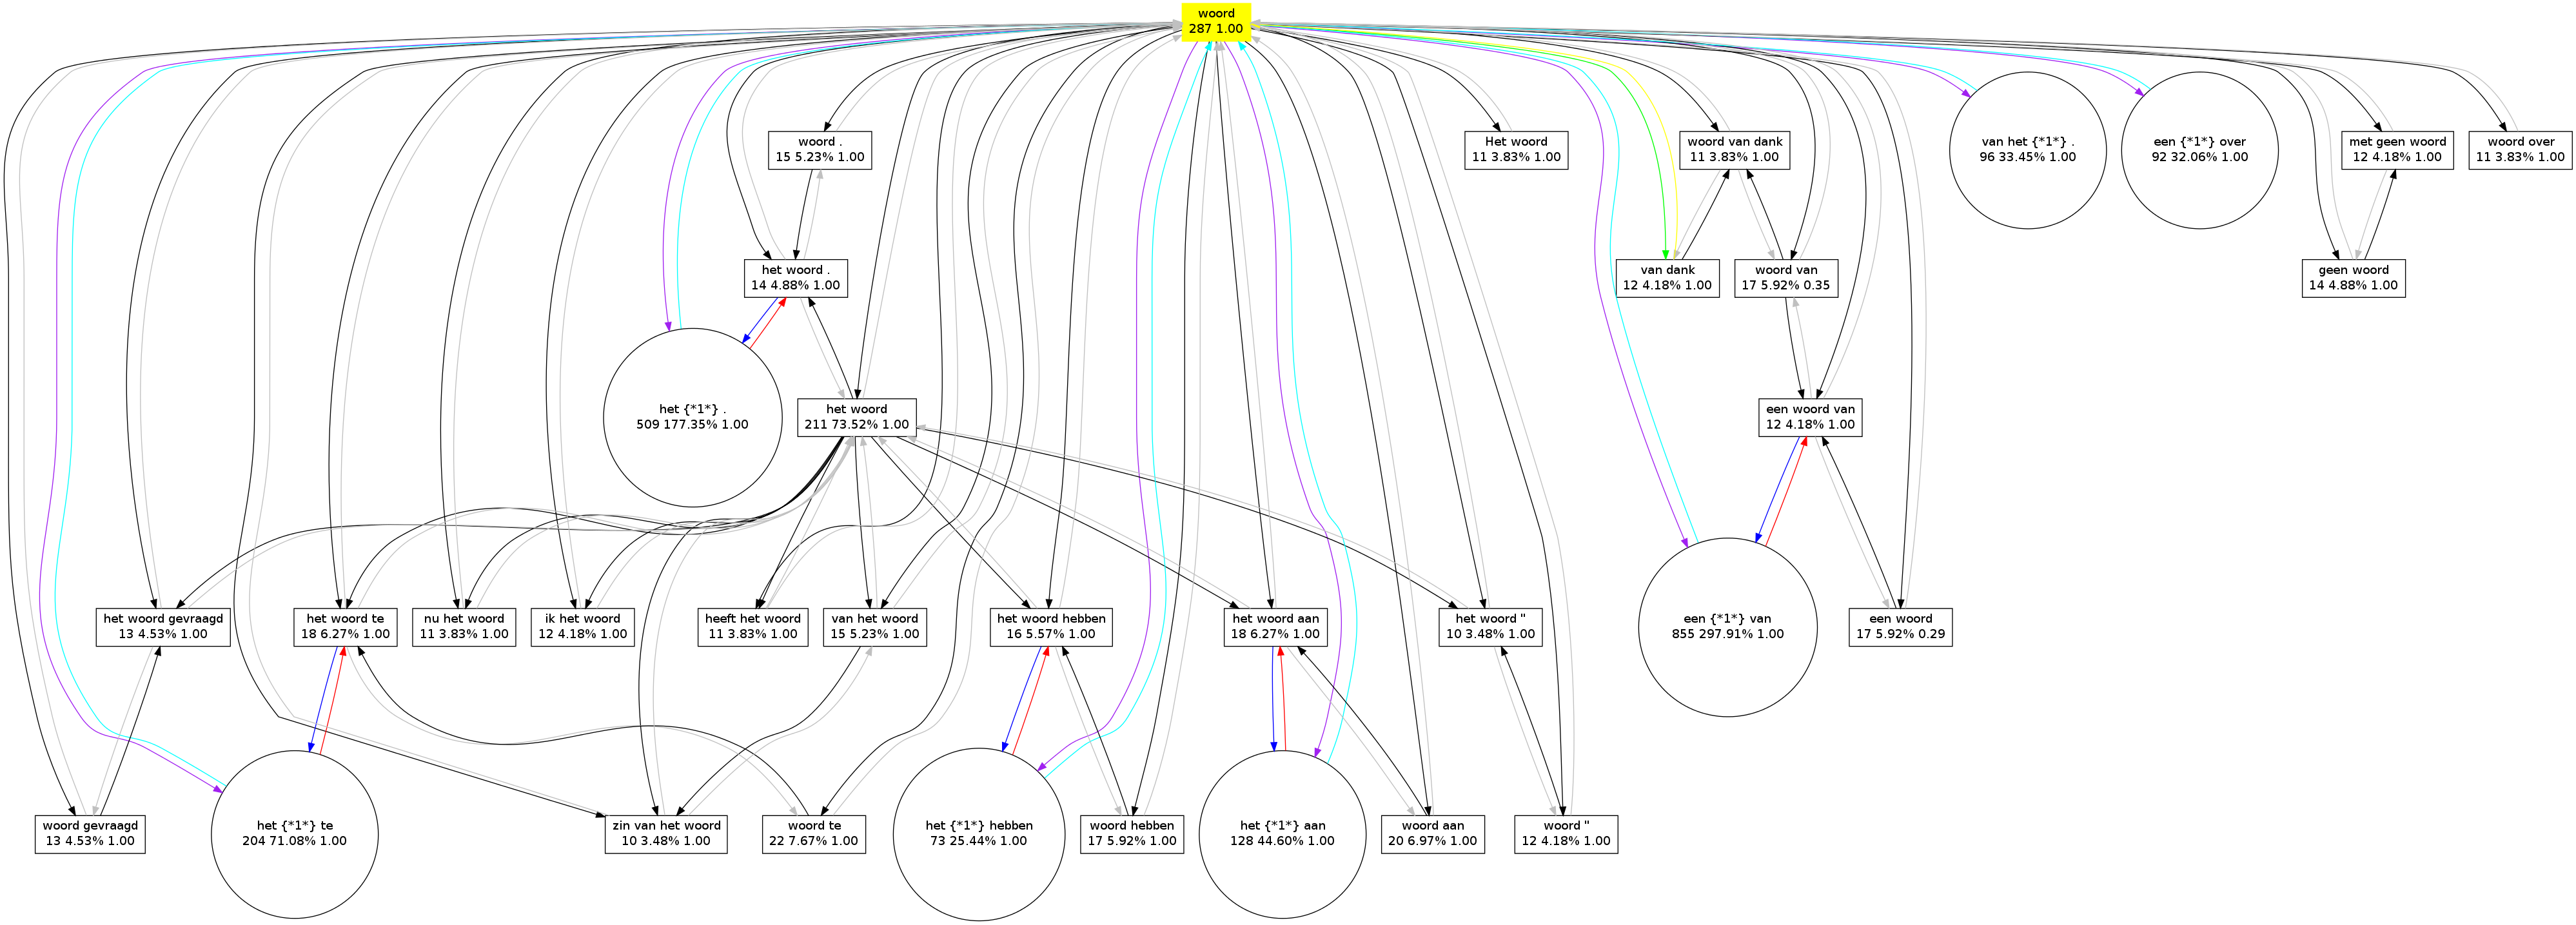
\includegraphics[width=170.0mm]{graph_woord_all.png}
\end{frame}

\begin{frame}{All relations: ``tot $*$ van''}
 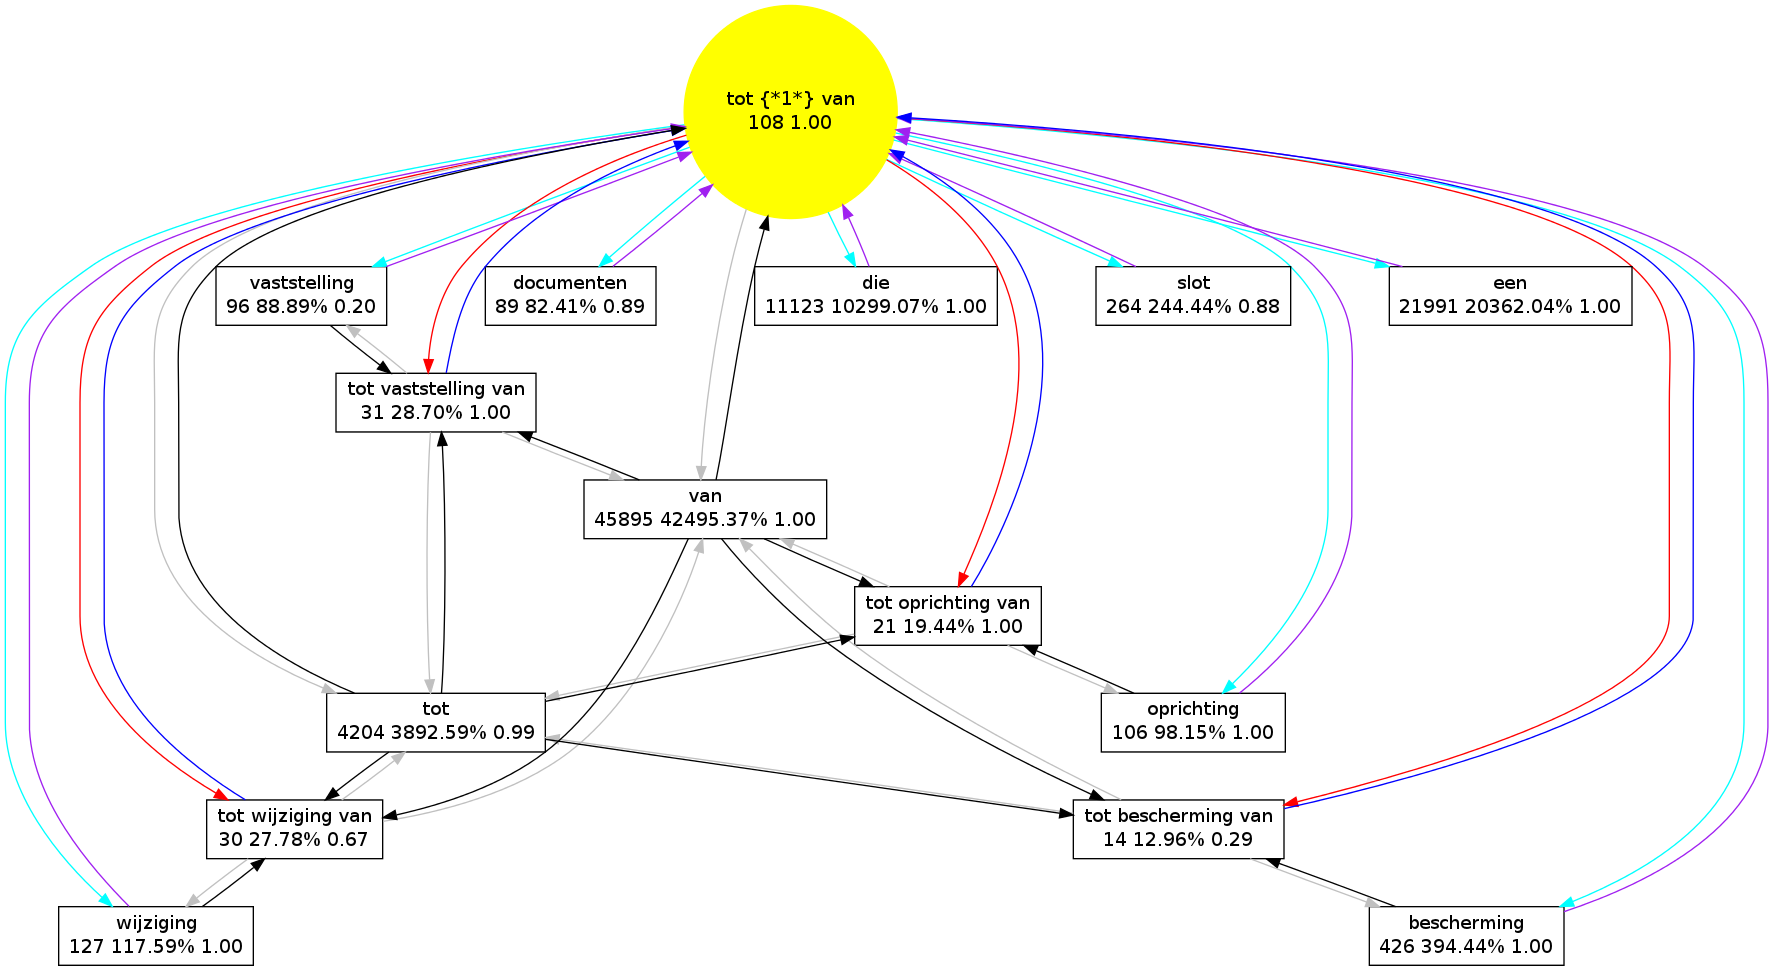
\includegraphics[width=140.0mm]{graph_totvan_all.png}
\end{frame}


%\begin{frame}{Using graph information in alignment}
% [HIER KOMT MOOI PLAATJE VAN HOE GRAAF-INFORMATIE GEBRUIKT KAN WORDEN OM ALIGNMENTS TE VERBETEREN (gewichten bijstellen)]
%\end{frame}

\section{The future}

\begin{frame}

	\begin{block}{Hypotheses}
		\begin{itemize}
			\item Constructions can be found efficiently in corpus data
			\item Graph-based relations can be used to constrain to ``good'' constructions
			\item Constructions can be aligned without resorting to word-alignments as a basis
			\item In MT, constructions (i.e. possibly with gaps) result in better translation than mere consecutive phrases
		\end{itemize}
	\end{block}

\end{frame}


\begin{frame}

	\begin{block}{Empirical Evaluation}	
		\begin{itemize}
			\item Evaluation of constructions in an MT setting
			\item Evaluation based on translation quality
			\begin{itemize}
				\item Comparison to human reference translations
			\end{itemize}
			\item Alternative use-case: Constructions in Language Modelling
		\end{itemize}
	\end{block}

\end{frame}

\begin{frame}

	\begin{block}{Use in linguistic studies}	
		\begin{itemize}
			\item Abstracting fully lexicalised constructions
			\begin{itemize}
				\item Finding semantic subclasses in constructions: ``from \emph{time-expression} to \emph{time-expression}''	
				\item Collapsing constructions with word disjunctions (``he/she/it'') or part-of-speech tags
			\end{itemize}
			\item Correlations with experimental findings
			\begin{itemize}
				\item Switch tasks, cloze tests, reaction times, ...
			\end{itemize}
			\item Modelling multilinguality			
			\begin{itemize}
				\item Parallel constructions
			\end{itemize}
			\item Software package for linguists?
		\end{itemize}	
	\end{block}

\end{frame}

\section{The End}

\begin{frame}

\raccoon

\begin{center}
\Large{Questions?}
\end{center}

\end{frame}


\end{document}  

